\section{Εισαγωγή}
Τα γραφήματα είναι δομές δεδομένων που συναντώνται συχνά κατά την επίλυση προβλημάτων. Η ευχέρεια προγραμματισμού αλγορίθμων που εφαρμόζονται πάνω σε γραφήματα είναι ουσιώδης. Καθώς μάλιστα συχνά ανακύπτουν προβλήματα για τα οποία έχουν διατυπωθεί αλγόριθμοι αποδοτικής επίλυσής τους η γνώση των αλγορίθμων αυτών αποδεικνύεται ισχυρός σύμμαχος στην επίλυση δύσκολων προβλημάτων. 

\section{Γραφήματα}
Ένα γράφημα ή γράφος (graph) είναι ένα σύνολο από σημεία που ονομάζονται κορυφές (vertices) ή κόμβοι (nodes) για τα οποία ισχύει ότι κάποια από αυτά είναι συνδεδεμένα απευθείας μεταξύ τους με τμήματα γραμμών που ονομάζονται ακμές (edges ή arcs). Συνήθως ένα γράφημα συμβολίζεται ως $G=(V,E)$ όπου $V$ είναι το σύνολο των κορυφών και $E$ είναι το σύνολο των ακμών.

Αν οι ακμές δεν έχουν κατεύθυνση τότε το γράφημα ονομάζεται μη κατευθυνόμενο (undirected) ενώ σε άλλη περίπτωση ονομάζεται κατευθυνόμενο (directed). Ένα πλήρες γράφημα (που όλες οι κορυφές συνδέονται απευθείας με όλες τις άλλες κορυφές) έχει $\frac{|V||V-1|}{2}$ ακμές ($|V|$ είναι το πλήθος των κορυφών του γραφήματος). Αν σε κάθε ακμή αντιστοιχεί μια τιμή τότε το γράφημα λέγεται γράφημα με βάρη. Το γράφημα του σχήματος \ref{fig:undirected_graph} είναι ένα μη κατευθυνόμενο γράφημα με βάρη.

\begin{figure}[ht]
\centering
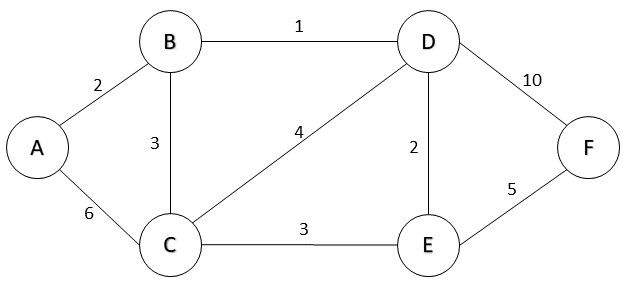
\includegraphics[width=100mm]{undirected_graph1.png}
\caption{Ένα μη κατευθυνόμενο γράφημα 8 κορυφών με βάρη στις ακμές του}
\label{fig:undirected_graph}
\end{figure}

\subsection{Αναπαράσταση γραφημάτων}
Δύο διαδεδομένοι τρόποι αναπαράστασης γραφημάτων είναι οι πίνακες γειτνίασης (adjacency matrices) και οι λίστες γειτνίασης (adjacency lists).

Στους πίνακες γειτνίασης διατηρείται ένας δισδιάστατος πίνακας $n \times n$ όπου $n$ είναι το πλήθος των κορυφών του γραφήματος. Για κάθε ακμή του γραφήματος που συνενώνει την κορυφή $i$ με την κορυφή $j$ εισάγεται στη θέση $i,j$ του πίνακα το βάρος της ακμής αν το γράφημα είναι με βάρη ενώ αν δεν υπάρχουν βάρη τότε εισάγεται η τιμή 1. Όλα τα υπόλοιπα στοιχεία του πίνακα λαμβάνουν την τιμή 0. Για παράδειγμα η πληροφορία του γραφήματος του σχήματος \ref{fig:undirected_graph} διατηρείται όπως φαίνεται στον πίνακα \ref{tbl:adjacency_table}.

% Please add the following required packages to your document preamble:
% \usepackage[table,xcdraw]{xcolor}
% If you use beamer only pass "xcolor=table" option, i.e. \documentclass[xcolor=table]{beamer}
\begin{table}[ht]
\centering
\begin{tabular}{|
>{\columncolor[HTML]{C0C0C0}}l |c|c|c|c|c|c|}
\hline
\cellcolor[HTML]{FFFFFF} & \cellcolor[HTML]{C0C0C0} A & \cellcolor[HTML]{C0C0C0} B & \cellcolor[HTML]{C0C0C0} C & \cellcolor[HTML]{C0C0C0}D  & \cellcolor[HTML]{C0C0C0} E  & \cellcolor[HTML]{C0C0C0} F \\ \hline
A                    & 0                             & 2                             & 6                             & 0                             & 0                            & 0                             \\ \hline
B                    & 2                             & 0                             & 3                             & 1                             & 0                            & 0                             \\ \hline
C                    & 6                             & 3                             & 0                             & 4                             & 3                            & 0                             \\ \hline
D                    & 0                             & 1                             & 4                             & 0                             & 2                            & 10                            \\ \hline
E                    & 0                             & 0                             & 3                             & 2                             & 0                            & 5                             \\ \hline
F                    & 0                             & 0                             & 0                             & 10                            & 5                            & 0                             \\ \hline
\end{tabular}
\label{tbl:adjacency_table}
\caption{Πίνακας γειτνίασης}
\end{table}

Στις λίστες γειτνίασης διατηρούνται λίστες που περιέχουν για κάθε κορυφή όλη την πληροφορία των συνδέσεών της με τους γειτονικούς του κόμβους. Για παράδειγμα το γράφημα του σχήματος \ref{fig:undirected_graph} μπορεί να αναπαρασταθεί με τις ακόλουθες 6 λίστες (μια ανά κορυφή). Κάθε στοιχείο της λίστας για τον κόμβο $v$ είναι ένα ζεύγος τιμών $(w,u)$ και αναπαριστά μια ακμή από τον κόμβο $v$ στον κόμβο $u$ με βάρος $w$, όπως φαίνεται στο πίνακα \ref{tbl:adjacency_list}.

\begin{table}[ht]
\centering
\begin{tabular}{|
>{\columncolor[HTML]{C0C0C0}}l |c|}
\hline
A & (2,B), (6,C)                \\ \hline
B & (2,A), (3,C), (1,D)         \\ \hline
C & (6,A), (3,B), (4,D), (3,E)  \\ \hline
D & (1,B), (4,C), (2,E), (10,F) \\ \hline
E & (3,C), (2,D), (5,F)         \\ \hline
F & (10,D), (5,E)               \\ \hline
\end{tabular}
\label{tbl:adjacency_list}
\caption{Λίστα γειτνίασης}
\end{table}

\subsection{Σημαντικοί αλγόριθμοι γραφημάτων}
Υπάρχουν πολλοί αλγόριθμοι που εφαρμόζονται σε γραφήματα προκειμένου να επιλύσουν ενδιαφέροντα προβλήματα που ανακύπτουν σε πρακτικές εφαρμογές. Οι ακόλουθοι αλγόριθμοι είναι μερικοί από αυτούς:
\begin{itemize}[noitemsep]
\item Αναζήτηση συντομότερων διαδρομών από μια κορυφή προς όλες τις άλλες κορυφές (Dijkstra)
\item Αναζήτηση συντομότερης διαδρομής από μια κορυφή προς μια άλλη κορυφή (Floyd Warshall)
\item Αναζήτηση κατά βάθος (Depth First Search)
\item Αναζήτηση κατά πλάτος (Breadth First Search)
\item Εντοπισμός ελάχιστου συνεκτικού δένδρου (Prim, Kruskal)
\item Τοπολογική ταξινόμηση (Topological Sort)
\item Εντοπισμός κυκλωμάτων Euler (Eulerian circuit)
\item Εντοπισμός ισχυρά συνδεδεμένων συνιστωσών (Stongly Connected Components)
\end{itemize} 

Στη συνέχεια θα παρουσιαστεί ο αλγόριθμος αναζήτησης των συντομότερων διαδρομών από μια κορυφή προς όλες τις άλλες κορυφές. Ο αλγόριθμος αυτός είναι γνωστός και ως αλγόριθμος του Dijkstra.
 
\section{Αλγόριθμος του Dijkstra για εύρεση συντομότερων διαδρομών}
Ο αλγόριθμος δέχεται ως είσοδο ένα γράφημα $G=(V,E)$ και μια κορυφή του γραφήματος $s$ η οποία αποτελεί την αφετηρία. Υπολογίζει για όλες τις κορυφές $v \in V$ το μήκος του συντομότερου μονοπατιού από την κορυφή $s$ στην κορυφή $v$. Για να λειτουργήσει σωστά θα πρέπει κάθε ακμή να έχει μη αρνητικό βάρος. Αν το γράφημα περιέχει ακμές με αρνητικό βάρος τότε μπορεί να χρησιμοποιηθεί ο αλγόριθμος των Bellman-Ford.

\subsection{Περιγραφή του αλγορίθμου}
Ο αλγόριθμος εντοπίζει τις συντομότερες διαδρομές προς τις κορυφές του γραφήματος σε σειρά απόστασης από την κορυφή αφετηρία. Σε κάθε βήμα του αλγορίθμου η αφετηρία και οι ακμές προς τις κορυφές για τις οποίες έχει ήδη βρεθεί συντομότερο μονοπάτι σχηματίζουν το υποδένδρο $S$ του γραφήματος. Οι κορυφές που είναι προσπελάσιμες με 1 ακμή από το υποδένδρο $S$ είναι υποψήφιες να αποτελέσουν την επόμενη κορυφή που θα εισέλθει στο υποδένδρο. Επιλέγεται μεταξύ τους η κορυφή που βρίσκεται στη μικρότερη απόσταση από την αφετηρία. Για κάθε υποψήφια κορυφή $u$ υπολογίζεται το άθροισμα της απόστασής της από την πλησιέστερη κορυφή $v$ του δένδρου συν το μήκος της συντομότερης διαδρομής από την αφετηρία $s$ προς την κορυφή $v$. Στη συνέχεια επιλέγεται η κορυφή με το μικρότερο άθροισμα. Όταν επιλεγεί η κορυφή που πρόκειται να προστεθεί στο δένδρο τότε προστίθεται στο σύνολο των κορυφών που απαρτίζουν το υποδένδρο $S$  και για κάθε μία από τις υποψήφιες κορυφές που συνδέονται με μια ακμή με την κορυφή που επιλέχθηκε ενημερώνεται η απόστασή της από το υποδένδρο εφόσον προκύψει μικρότερη τιμή.

\paragraph{Ψευδοκώδικας}
Το σύνολο $S$ περιέχει τις κορυφές για τις οποίες έχει προσδιοριστεί η συντομότερη διαδρομή από την κορυφή $s$ ενώ το διάνυσμα $d$ περιέχει τις αποστάσεις από την κορυφή $s$ \\
1. Αρχικά $S={s}$, $d_s=0$ και για όλες τις κορυφές $i \neq s, d_i=+\infty$ \\
2. Μέχρι να γίνει $S=V$ \\
3. Εντοπισμός του στοιχείου $v \notin S$ με τη μικρότερη τιμή $d_v$ και προσθήκη του στο $S$ \\
4. Για κάθε ακμή από την κορυφή $v$ στην κορυφή $u$ με βάρος $w$ ενημερώνεται η τιμή $d_u$ έτσι ώστε: \\
\centerline{$d_u=min(d_u, d_v+w)$}
5. Επιστροφή στο βήμα 2.

\paragraph{Εκτέλεση του αλγορίθμου}
Στη συνέχεια ακολουθεί παράδειγμα εκτέλεσης του αλγορίθμου για το γράφημα του σχήματος \ref{fig:undirected_graph}.

\begin{table}[ht]
\centering
\label{my-label}
\begin{tabular}{|c|p{5cm}|}
\hline
$S=\{A\},d_A=0,d_B=2,d_C=6,d_D=\infty,d_E=\infty,d_F=\infty $ & Από το $S$ μπορούμε να φτάσουμε στις κορυφές 2 και 3 με μήκος διαδρομής 2 και 6 αντίστοιχα. Επιλέγεται η κορυφή 2. \\ \hline
$S=\{A,B\}, d_A=0, d_B=2, d_C=5, d_D=3, d_E=\infty, d_F=\infty$ & Από το $S$ μπορούμε να φτάσουμε στις κορυφές C και D με μήκος διαδρομής 5 και 3 αντίστοιχα. Επιλέγεται η κορυφή D.\\ \hline
$S= \{A,B,D\},d_A=0,d_B=2,d_C=5,d_D=3,d_E=5,d_F=13$  & Από το $S$ μπορούμε να φτάσουμε στις κορυφές C, E και F με μήκος διαδρομής 5, 5 και 13 αντίστοιχα. Επιλέγεται (με τυχαίο τρόπο) ανάμεσα στις κορυφές C και E η κορυφή E. \\ \hline
$S=\{A,B,D,C\},d_A=0,d_B=2,d_C=5,d_D=3,d_E=5,d_F=13$ & Από το $S$ μπορούμε να φτάσουμε στις κορυφές E και F με μήκος διαδρομής 5 και 13 αντίστοιχα. Επιλέγεται η κορυφή E. \\ \hline
$S=\{A,B,D,C,E\},d_A=0,d_B=2,d_C=5,d_D=3,d_E=5,d_F=10$ & Η μοναδική κορυφή στην οποία μένει να φτάσουμε από το $S$ είναι η κορυφή F και το μήκος της συντομότερης διαδρομής από την A στην F είναι 10. \\ \hline
\multicolumn{2}{|c|}{$S=\{A,B,D,C,E,F\},d_A=0,d_B=2,d_C=5,d_D=3,d_E=5,d_F=10$ } \\ \hline
\end{tabular}
\caption{Αναλυτική εκτέλεση του αλγορίθμου}
\end{table}

\begin{table}[ht]
\centering
\begin{tabular}{|c|c|c|c|c|c|c|}
\hline
Σύνολο $S$        & A & B      & C      & D      & E      & F      \\ \hline
$\{\}$            & 0 & $\infty$ & $\infty$ & $\infty$ & $\infty$ & $\infty$ \\ \hline
$\{A\}$           & 0 & 2      & 6      & $\infty$ & $\infty$ & $\infty$ \\ \hline
$\{A,B\}$         & 0 & 2      & 5      & 3      & $\infty$ & $\infty$ \\ \hline
$\{A,B,D\}$       & 0 & 2      & 5      & 3      & 5      & 13     \\ \hline
$\{A,B,D,C\}$     & 0 & 2      & 5      & 3      & 5      & 13     \\ \hline
$\{A,B,D,C,E\}$   & 0 & 2      & 5      & 3      & 5      & 13     \\ \hline
$\{A,B,D,C,E,F\}$ & 0 & 2      & 5      & 3      & 4      & 10     \\ \hline
\end{tabular}
\caption{Συνοπτική εκτέλεση του αλγορίθμου}
\label{my-label}
\end{table}

Συνεπώς ισχύει ότι: 
\begin{itemize}[noitemsep]
\item Για την κορυφή A η διαδρομή αποτελείται μόνο από τον κόμβο A και έχει μήκος 0.
\item Για την κορυφή B η διαδρομή είναι η A-B με μήκος 2.
\item Για την κορυφή C η διαδρομή είναι η A-B-C με μήκος 5.
\item Για την κορυφή D η διαδρομή είναι η A-B-D με μήκος 3.
\item Για την κορυφή E η διαδρομή είναι η A-B-D-E με μήκος 5.
\item Για την κορυφή F η διαδρομή είναι η A-B-D-E-F με μήκος 10.
\end{itemize}

\paragraph{Απόδοση του αλγορίθμου}

Η ταχύτητα εκτέλεσης του αλγορίθμου εξαρτάται από τις δομές δεδομένων που χρησιμοποιούνται για να αναπαρασταθεί το γράφημα. Γενικά, πρόκειται για έναν εξαιρετικά γρήγορο αλγόριθμο με πολυπλοκότητα χειρότερης περίπτωσης $O(|E| log |V|)$, όπου $|E|$ είναι ο αριθμός των ακμών και $|V|$ ο αριθμός των κορυφών του γραφήματος.

\subsection{Κωδικοποίηση του αλγορίθμου}


\section{Παραδείγματα}

\subsection{Παράδειγμα 1}

\subsection{Παράδειγμα 2}


\section{Ασκήσεις}
\begin{enumerate}
\item 
\item 
\end{enumerate}

\begin{thebibliography}{9}
\end{thebibliography}

